%%%%%%%%%%%%%%%%%%%%%%%%%%%%%%%%%%%%%%%%%%%%%%%%%%%%%%%%%%%%%%%%%%%%%%%
%%%%%%%%%%%%%%%%%%%%%%%%%%%%%%%%%%%%%%%%%%%%%%%%%%%%%%%%%%%%%%%%%%%%%%% 
%%%%%%%%%%%       								 Preamble				         	                                                        %%%%%%%%%% 
%%%%%%%%%%%%%%%%%%%%%%%%%%%%%%%%%%%%%%%%%%%%%%%%%%%%%%%%%%%%%%%%%%%%%%% 
%%%%%%%%%%%%%%%%%%%%%%%%%%%%%%%%%%%%%%%%%%%%%%%%%%%%%%%%%%%%%%%%%%%%%%% 
\documentclass[10pt]{beamer}
\usepackage{setspace}
\usepackage{color}
\usepackage{amsmath,lmodern}
\usepackage{hyperref}
\usepackage{graphicx}
\usepackage{multirow}
\usepackage{tikz}
\usetikzlibrary{fit,shapes.misc}
\usepackage{pdflscape}
\usepackage{amsmath}
\usepackage{lscape}
\usepackage{multirow}
\usepackage{enumerate}
\usepackage{mathtools}
\usepackage{epstopdf}
\usepackage{pdfpages}
\usepackage{bm}
\usepackage{appendixnumberbeamer}
\usepackage{color,soul}
\usepackage{grffile}
\usepackage{float}
\usepackage{relsize}
\usepackage{tcolorbox}
\newcounter{nodemarkers}
\usepackage{tikz}
\newcommand{\toplinesmall}{%
  \tikz[remember picture,overlay] {%
    \draw[blue,thick] ([yshift=-1cm, xshift=.9cm]current page.north west)
             -- ([yshift=-1cm,xshift=3.6cm]current page.north west);}}
             
\newcommand{\toplinemedium}{%
  \tikz[remember picture,overlay] {%
    \draw[blue,thick] ([yshift=-1cm, xshift=.9cm]current page.north west)
             -- ([yshift=-1cm,xshift=6.2cm]current page.north west);}}
 
 \newcommand{\toplinelarge}{%
  \tikz[remember picture,overlay] {%
    \draw[blue,thick] ([yshift=-1cm, xshift=.9cm]current page.north west)
             -- ([yshift=-1cm,xshift=8.9cm]current page.north west);}}           
             
 \newcommand{\toplinexlarge}{%
  \tikz[remember picture,overlay] {%
    \draw[blue,thick] ([yshift=-1cm, xshift=.9cm]current page.north west)
             -- ([yshift=-1cm,xshift=12cm]current page.north west);}}                       
             
\setbeamertemplate{footline}
{
  \leavevmode%
  \hbox{%
  \begin{beamercolorbox}[wd=.333333\paperwidth,ht=2.25ex,dp=1ex,center]{author in head/foot}%
    \usebeamerfont{author in head/foot}{\textcolor{blue}{ECON712}}
  \end{beamercolorbox}%
  \begin{beamercolorbox}[wd=.333333\paperwidth,ht=2.25ex,dp=1ex,center]{title in head/foot}%
    \usebeamerfont{title in head/foot}{\textcolor{blue}{Winter 2026}}
  \end{beamercolorbox}%
  \begin{beamercolorbox}[wd=.333333\paperwidth,ht=2.25ex,dp=1ex,right]{date in head/foot}%
    \usebeamerfont{date in head/foot}{\textcolor{blue}{Lecture 9, 10 \: \: \: \: \: \: \: }
    \insertframenumber{} / \inserttotalframenumber\hspace*{2ex}} 
  \end{beamercolorbox}}%
  \vskip0pt%
}
\newtheorem{proposition}[theorem]{Proposition}

\newcommand\marktopleft[1]{%
    \tikz[overlay,remember picture] 
        \node (marker-#1-a) at (-0.2,1.2ex) {};%
}
\newcommand\markbottomright[1]{%
    \tikz[overlay,remember picture] 
        \node (marker-#1-b) at (0.16,-1ex) {};%
    \tikz[overlay,remember picture,thick,inner sep=4pt]
        \node[draw,rectangle,rounded corners, blue, fit=(marker-#1-a.center) (marker-#1-b.center)] {};%
}

\setbeamertemplate{caption}{\raggedright\insertcaption\par}
\setbeamertemplate{itemize items}[ball]
\setbeamertemplate{itemize subitem}[triangle]
\setbeamertemplate{itemize subsubitem}[triangle]
\tcbset{colframe=white,colback=white,nobeforeafter}
\beamertemplatenavigationsymbolsempty
\addtobeamertemplate{frametitle}{\vspace*{0.19cm}}{\vspace*{0cm}}


%%%%%%%%%%%%%%%%%%%%%%%%%%%%%%%%%%%%%%%%%%%%%%%%%%%%%%%%%%%%%%%%%%%%%%%
%%%%%%%%%%%%%%%%%%%%%%%%%%%%%%%%%%%%%%%%%%%%%%%%%%%%%%%%%%%%%%%%%%%%%%% 
%%%%%%%%%  									    Define Title									                                       %%%%%%%%%
%%%%%%%%%%%%%%%%%%%%%%%%%%%%%%%%%%%%%%%%%%%%%%%%%%%%%%%%%%%%%%%%%%%%%%%
%%%%%%%%%%%%%%%%%%%%%%%%%%%%%%%%%%%%%%%%%%%%%%%%%%%%%%%%%%%%%%%%%%%%%%% 
\title{ECON 712: Applied Econometrics} 
\author{Lecture 9, 10: Linear Regression and the CEF}
\date{}
\AtBeginSection[]
{
 \begin{frame}<beamer>
 \tableofcontents[currentsection]
 \end{frame}
}
%%%%%%%%%%%%%%%%%%%%%%%%%%%%%%%%%%%%%%%%%%%%%%%%%%%%%%%%%%%%%%%%%%%%%%%
%%%%%%%%%%%%%%%%%%%%%%%%%%%%%%%%%%%%%%%%%%%%%%%%%%%%%%%%%%%%%%%%%%%%%%% 
%%%%%%%% 						     				Document								                                                %%%%%%%%
%%%%%%%%%%%%%%%%%%%%%%%%%%%%%%%%%%%%%%%%%%%%%%%%%%%%%%%%%%%%%%%%%%%%%%%
%%%%%%%%%%%%%%%%%%%%%%%%%%%%%%%%%%%%%%%%%%%%%%%%%%%%%%%%%%%%%%%%%%%%%%% 
\begin{document}
\setbeamercovered{transparent}

\begin{frame}
\maketitle
\end{frame}

\section{FWL Theorem-- Using Vector Algebra}

\begin{frame}
\frametitle{\: \: \: Linear Transformations} 
\toplinelarge
\begin{itemize}
\item Subtracting a constant $\bm{\iota}\bar{x}$ from regressors when the constant term is included
\end{itemize}
\begin{figure}
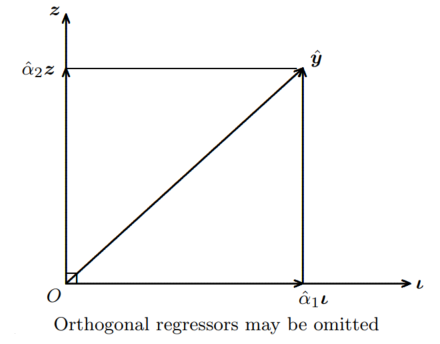
\includegraphics[scale=0.55]{average.png}
\end{figure}
\end{frame}

\begin{frame}
\frametitle{\: \: \: Linear Transformations} 
\toplinelarge
\begin{itemize}
\item For a general regression where regressors are partitioned: $\bm{X}=[\bm{X_1} \: \bm{X_2}]$, $\bm{X_1}$ is an $nxk_1$, $\bm{X_2}$ is an $nxk_2$ ; $\bm{\beta_1}$ is $k_1x1$, $\bm{\beta_2}$ is $k_2x1$, and $k_1+k_2=k$
\begin{eqnarray*}
\bm{y}=\bm{X_1} \bm{\beta_1}+\bm{X_2} \bm{\beta_2} +u
\end{eqnarray*}
the OLS/MM estimator has the following properties:
\begin{eqnarray*}
\begin{array}{ll}
\bm{y}=\bm{X_1} \bm{\hat{\beta}_1}+\bm{X_2} \bm{\hat{\beta}_2}+\bm{\hat{u}} \\[1.4ex]
\bm{y}=\bm{X_1} \bm{\hat{\alpha}_1}+\bm{Z} \bm{\hat{\beta}_2}+\bm{\hat{u}}  \\[1.4ex]
\end{array}
\end{eqnarray*} 
where $\bm{Z}=\bm{X_2}-\bm{X_1} \: \bm{A}$ and $\bm{A}$ is a $k_1xk_1$ non-singular matrix
\end{itemize}
\end{frame}

\begin{frame}
\frametitle{\: \: \: Linear Transformations} 
\toplinelarge
\begin{itemize}
\item In addition, if the transformation results in:
\begin{eqnarray*}
 \langle \bm{X_1},\bm{Z} \rangle =\bm{X_1}^{T} \: \bm{Z}=\bm{0}
 \end{eqnarray*}
 then,
 \begin{eqnarray*}
\bm{y}=\bm{Z} \bm{\hat{\beta}_2} +\bm{\hat{\epsilon}}
\end{eqnarray*}
\item This is the basis of the FWL theorem we studied in ECON 312:
\begin{itemize}
\vspace{0.11in}
\item Let $\bm{Z}=\bm{X_2}-\bm{P_{X_1}}\bm{X_2}=\bm{M_{X_1} \: X_2}$, then
 \begin{eqnarray*}
\bm{P_Z}\bm{y}=\bm{Z} \bm{\hat{\beta}_2} 
\end{eqnarray*}
\end{itemize}
\item Note that residuals of this regression are not the same as the residuals of the original regression
\end{itemize}
\end{frame}

\begin{frame}
\frametitle{\: \: \: FWL-- with vector algebra} 
\toplinelarge
\begin{itemize}
\item Suppose that the OLS/MM estimator results in:
\begin{eqnarray*}
\bm{y}=\bm{X_1} \bm{\hat{\beta}_1}+\bm{X_2} \bm{\hat{\beta}_2}+\bm{\hat{u}}
\end{eqnarray*}
and define $\bm{Z}=\bm{M_{X_1} \: X_2}$, $\bm{\widetilde{y}}=\bm{M_{X_1} \: y}$, then:
\begin{eqnarray*}
\begin{array}{ll}
\bm{P_Z} \: \bm{\widetilde{y}}=\bm{Z} \bm{\hat{\beta}_2}   &\text{ , and} \\[1.2ex]
\bm{M_Z}\: \bm{\widetilde{y}}=\bm{\hat{u}}
\end{array}
\end{eqnarray*}
\item This yields the following equation, where $\bm{\hat{\beta}_2}$ denotes the OLS/MM estimator:
\begin{eqnarray*}
\bm{\widetilde{y}}=\bm{Z} \bm{\hat{\beta}_2}+\bm{\hat{u}}
\end{eqnarray*}
\end{itemize}
\end{frame}

\begin{frame}
\frametitle{\: \: \: Goodness of Fit} 
\toplinemedium
\begin{itemize}
\item Recall that, by Pythagoras' Theorem:  
\begin{eqnarray*}
TSS=\|\bm{y}\|^2=\|\bm{P_X \: y}\|^2+\|\bm{M_X \: y}\|^2=ESS+SSR
\end{eqnarray*}
\vspace{0.11in}
\item We use this result to obtain two goodness of fit measures:
\begin{eqnarray*}
R_u^2= \frac{\|\bm{P_X \: y}\|^2}{\|\bm{y}\|^2} \\[1.4ex]
R_c^2= \frac{\|\bm{P_X \: M_{\iota} \: y}\|^2}{\|\bm{ M_{\iota} \: y}\|^2} 
\end{eqnarray*}
\item Note that the $R^2$-centered is preferred, but it can only be interpreted when the constant term is included in the regression
\end{itemize}
\end{frame}

\section{CEF and Linear Regression}

\begin{frame}
\frametitle{\: \: \: Why Linear Regression?} 
\toplinelarge
\begin{itemize}
\item Suppose that the population CEF is linear and has the following functional form:
\begin{eqnarray*}
\mathbb{E}[y_i|\bm{X}_i]=\bm{X}_i^T \bm{\beta}^* \text{   (MHE notation)}
\end{eqnarray*}
\begin{itemize}
\item by the CEF Decomposition Theorem: 
\begin{eqnarray*}
\mathbb{E}[\bm{X}_i (y_i-\mathbb{E}[y_i|\bm{X}_i])]=\bm{0}
\end{eqnarray*}
\item Substituting for the linear CEF:
\begin{eqnarray*}
\mathbb{E}[\bm{X}_i (y_i-\bm{X}_i^T \bm{\beta}^*]=\bm{0}
\end{eqnarray*}
\item Solving for $\bm{\beta}^*=\mathbb{E}[\bm{X}_i \: \bm{X}^T_i ]^{-1} \mathbb{E}[\bm{X}_i \: y_i]=\bm{\beta}^{OLS}$
\end{itemize}
\vspace{0.11in}
\item Interpretation: OLS solves the same problem as the linear CEF
\end{itemize}
\end{frame}

\begin{frame}
\frametitle{\: \: \: Why Linear Regression?}
\toplinelarge
\begin{itemize}
\item What if the CEF is \textcolor{blue}{not linear}?
\begin{enumerate}
\vspace{0.11in}
\item By definition, $\bm{\beta}^{OLS}$ provides the best linear prediction of $y_i$:
\[
\bm{\beta}^{OLS}
= \underset{b}{argmin}\; \mathbb{E}\!\left[(y_i-\bm{X}_i^T \bm{b})^2\right]
\]

\item $\bm{\beta}^{OLS}$ is the best linear approximation to the CEF:
\[
\bm{\beta}
=  \underset{b}{argmin}\; \mathbb{E}\!\left[(\mathbb{E}[y_i|\bm{X}_i]-\bm{X}_i^T \bm{b})^2\right]
\]

\begin{itemize}
\item Proof: by FOC
\[
\mathbb{E}[\bm{X}_i (\mathbb{E}[y_i|\bm{X}_i]-\bm{X}_i^T \bm{\beta})]=\bm{0} \Rightarrow
\]

\[
\bm{\beta}=\mathbb{E}[\bm{X}_i \bm{X}_i^T ]^{-1}
\mathbb{E}[\bm{X}_i y_i]
=\bm{\beta}^{OLS}
\]
\vspace{0.11in}
where the last line uses the CEF decomposition property.
\end{itemize}

\end{enumerate}
\end{itemize}

\end{frame}

\begin{frame}
\frametitle{\: \: \: Linear Regression and CEF} 
\toplinelarge
\begin{figure}
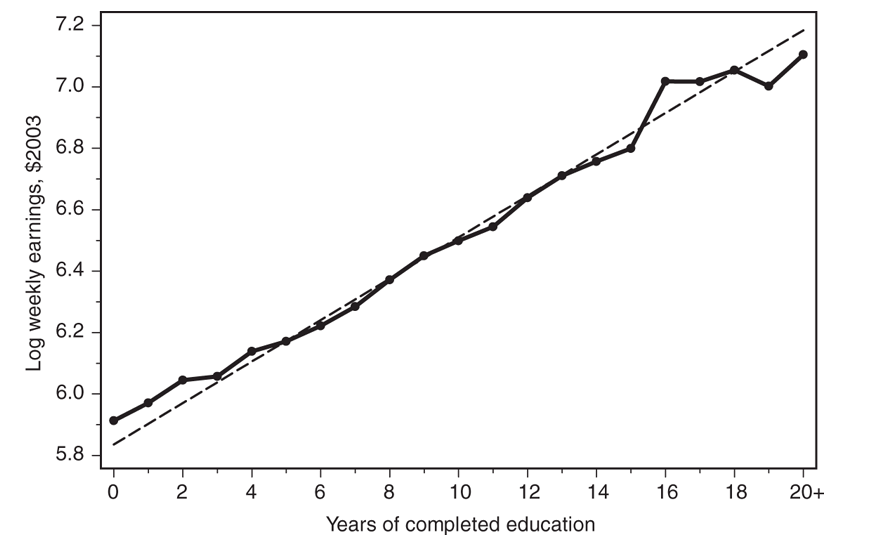
\includegraphics[scale=0.6]{educ_wages_linear.png}
\end{figure}
\end{frame}

\begin{frame}
\frametitle{\: \: \: Finite Sample Properties of OLS} 
\toplinelarge
\begin{itemize}
\item Under strict exogeneity, $\mathbb{E}[\bm{u}|\bm{X}]=\bm{0}$, OLS/MM is unbiased:
\begin{eqnarray*}
\begin{array}{rl}
\bm{\hat{\beta}}^{ols}&=(\bm{X}^T \bm{X})^{-1} \bm{X}^T \bm{y} \\[1.2ex]
 \bm{\hat{\beta}}^{ols}  &=\bm{\beta}+(\bm{X}^T \bm{X})^{-1} \bm{X}^T \bm{u}  \\[1.2ex]
                                 \mathbb{E}[\bm{\hat{\beta}}^{ols}|\bm{X}] &=\bm{\beta}\underbrace{=}_{\text{by LIE}}  \mathbb{E}[\bm{\hat{\beta}}^{ols}]
\end{array}
\end{eqnarray*}
\item Pre-determinedness, $\mathbb{E}[u_i|x_{1i}, \cdot , x_{ki}]=0$, is not enough
\vspace{0.11in}
\item The linear CEF has to be correctly specified
\end{itemize}
\end{frame}

\end{document}